% Source: graduate-coursework/Research/How_to_write/00_Contrastive_Synthesis.tex
% Description: \textbf{Expressivism.

\documentclass[border=4pt]{standalone}
\usepackage{newtxtext,newtxmath}
\usepackage{tikz}
\usetikzlibrary{arrows.meta,positioning,shapes.geometric,calc,decorations.pathreplacing}

\definecolor{garnet}{HTML}{73000A}
\definecolor{atlantic}{HTML}{466A9F}
\definecolor{congaree}{HTML}{1F414D}
\definecolor{horseshoe}{HTML}{65780B}
\definecolor{rose}{HTML}{CC2E40}
\definecolor{honeycomb}{HTML}{A49137}
\definecolor{warmgrey}{HTML}{676156}
\definecolor{black90}{HTML}{363636}
\definecolor{black70}{HTML}{5C5C5C}
\definecolor{black50}{HTML}{A2A2A2}
\definecolor{black30}{HTML}{C7C7C7}
\definecolor{black10}{HTML}{ECECEC}
\definecolor{sandstorm}{HTML}{FFF2E3}

\begin{document}
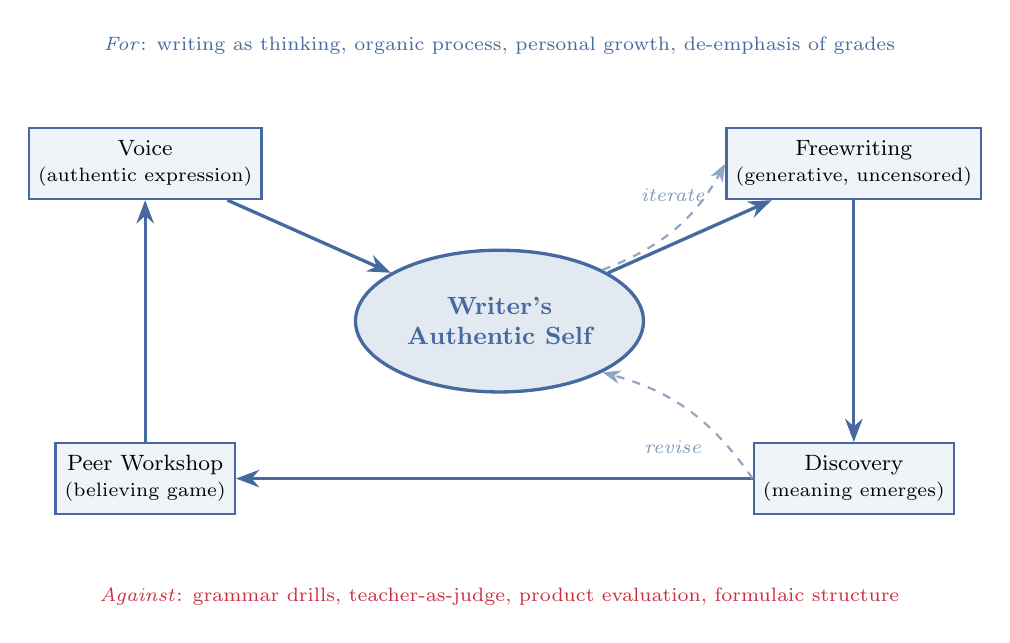
\begin{tikzpicture}[
    every node/.style={font=\footnotesize},
    box/.style={rectangle, draw=atlantic, thick, fill=atlantic!8,
        minimum width=2.2cm, minimum height=0.9cm, align=center, font=\footnotesize},
]
% Central writer
\node[ellipse, draw=atlantic, very thick, fill=atlantic!15,
    minimum width=3cm, minimum height=1.8cm, align=center, font=\small\bfseries,
    text=atlantic] (self) at (0,0) {Writer's\\Authentic Self};

% Surrounding process nodes in a cycle
\node[box] (free) at (4.5, 2) {Freewriting\\{\scriptsize (generative, uncensored)}};
\node[box] (discover) at (4.5, -2) {Discovery\\{\scriptsize (meaning emerges)}};
\node[box] (voice) at (-4.5, 2) {Voice\\{\scriptsize (authentic expression)}};
\node[box] (peer) at (-4.5, -2) {Peer Workshop\\{\scriptsize (believing game)}};

% Cycle arrows
\draw[-{Stealth}, very thick, atlantic] (self) -- (free);
\draw[-{Stealth}, very thick, atlantic] (free) -- (discover);
\draw[-{Stealth}, very thick, atlantic] (discover) -- (peer);
\draw[-{Stealth}, very thick, atlantic] (peer) -- (voice);
\draw[-{Stealth}, very thick, atlantic] (voice) -- (self);

% Revision spiral arrow
\draw[-{Stealth}, thick, atlantic!60, dashed] (discover.west) to[bend right=20] (self.south east);
\node[font=\scriptsize\itshape, text=atlantic!70] at (2.2, -1.6) {revise};

% Multiple drafts annotation
\draw[-{Stealth}, thick, atlantic!60, dashed] (self.north east) to[bend right=20] (free.west);
\node[font=\scriptsize\itshape, text=atlantic!70] at (2.2, 1.6) {iterate};

% Anti-CTR annotations
\node[font=\scriptsize, text=rose, align=center] at (0, -3.5)
    {\textit{Against}: grammar drills, teacher-as-judge, product evaluation, formulaic structure};
\node[font=\scriptsize, text=atlantic, align=center] at (0, 3.5)
    {\textit{For}: writing as thinking, organic process, personal growth, de-emphasis of grades};
\end{tikzpicture}
\end{document}
